
\section{Experiments}

\subsection{Datasets and Protocols}
In this work, we measure the model performance on the Tripitaka Koreana in Han (TKH) Dataset and the Multiple Tripitaka in Han (MTH) Dataset~\cite{tkhmth}. Following~\cite{jla},
we use the combined version of TKH and MTH2200, which is named MTHv2. Specifically, the MTHv2 dataset provides line-level annotation, character-level annotation, and ``boundary lines'' which include reading order information. In this work, we mainly use the line-level annotation which takes the minimum cost to obtain. 

Protocol-wise, we mainly evaluate the overall performance of our method on the full testing set, following the exact split from ~\cite{jla}, which randomly split the MTHv2 dataset into the training set and the testing set with the ratio of 3:1. It is important to note that our training and test sets are kept completely consistent with ~\cite{jla}. We did not use any additional data such as synthetic data or pre-trained models
Besides the benchmarking, we conduct extensive ablative and behavior analysis to validate the proposed approach.

\subsection{Implementation details}
The code is implemented based on the OpenCCD code base~\cite{vsdf}. The input image is resized to $32$ pixels by width and center padded to $32\times 320$ image. The model is trained for $128$ epochs with batch size set to $64$ from scratch.

The experiments are conducted on a virtual machine with Pytorch-$1.12.1$, TorchVision-$0.13.1$ CUDA-$11.2$, and Ubuntu $22.04$. Training from scratch using an Nvidia RTX 4090 GPU would typically take around 10 hours to complete 128 epochs. Depending on the model, when the batch size is set to $64$, the GPU memory usage is about 11-21$GB$. The models, codes, and documents are released on~\url{https://github.com/makaspacex/spindlenet}.

\subsection{Open-set Comparison with SOTA}

This section discusses the novel characters recognition capability of the proposed model. Since the new characters are mainly distributed in the tail, we discuss the performance change of the tail class and report the main performance indicators of the new characters.
\subsubsection{Per-class Performance Analysis}
\input{figures/freqvsimprovement.tex}
This provides per-class performance change analysis to provide more insight on the improving pattern. 
The overall trend is shown in Fig.\ref{fig:freqvsimprovement}.
The blue line is drawn in descending order of character frequency. Under the condition of ensuring character alignment, the red line draws the improvement in accuracy and the reduction in intra-class variance respectively. Since the original data changes greatly and the trend cannot be seen, the red line is smoothed using the moving average method. The window size of the moving average method is 250. It can be seen that the performance improvement of the head class is significantly smaller than that of the tail class, both in terms of accuracy and intra-class variance. This proves that SpindleNet has better feature extraction capabilities, thereby improving the performance of the tail class. Furthermore, the performance of new characters in the tail class has also been improved, and the specific data will be shown next.

% You claimed it would improve tail classes, now prove it. 

%Also try to give a description of the behavior of the head classes, try to give a few assumptions, and leave the proof as homework to the readers.

\subsubsection{Novel Characters Performance on MTHv2}
\begin{table}[]
    \centering
    \caption{Novel characters  performentce comparison to State of The Art methods on the MTHv2~\cite{jla} dataset. LA refers to Line Accuracy and Acc refers to character accuracy.}
    \begin{tabular}{c|c|c|ccc}
        \hline
         Name & Venue & AR & CR & LA & Acc \\
         \hline
         VSDF*\cite{vsdf}& CVPR' 22  &77.56 &81.65 &29.08 & 51.40 \\
         \hline
         Ours&- & \textbf{79.31} &\textbf{82.96}  & \textbf{29.26} & \textbf{52.96} \\
        \hline
    \end{tabular}
    \label{tab:zero_shot}
\end{table}
We report the performances of samples that contain unseen characters to give an estimation of how well the proposed modules handle the unseen characters in Table.~\ref{tab:zero_shot}. In the base model, the accuracy of new characters is \textbf{51.40}, while in the spindle network, the accuracy of new characters is \textbf{52.96}. When calculating the accuracy of new characters, more stringent standards are used. Specifically, no alignment operation is performed before calculation. Only when the predicted characters are consistent with the characters in GT at the corresponding positions, the characters are judged to be correct.
When a line of text contains new characters, the line of text is used to calculate $AR$, $CR$, and $LA$.
In Table.~\ref{tab:zero_shot}, SpindleNet achieves SOTA results in new character recognition performance, both in $AR$, $CR$, $ACC$ and $LA$. In summary, we have proven the highly consistent relationship between new characters and tail classes, and the effectiveness of SpindleNet in new character recognition.

\subsection{Close-set Comparison with SOTA}
This section discusses the close-set recognition capability of the proposed model. We report the performance of the proposed model on mainstream indicators in Table 2. The proposed model achieved SOTA in each indicator of the closed set test. Specifically, the performance of AR, CR and LA are 94.21, 95.27 and 70.77 respectively. According to the observation in Fig.\ref{fig:freqvsimprovement}, the performance improvement mainly comes from the tail class.

\input{tables/sota}

\subsection{Ablative Studies}
We first conduct module-level ablative experiments to validate the effectiveness of the proposed spindle network. Then, we provide an extended architecture-level ablative analysis, discussing various other possible designs and why they are less feasible than the proposed spindle-shaped network. 

\subsubsection{Module-level Ablative}

\begin{figure}[!t]
    \begin{center}
    \includegraphics[width=1.0\linewidth]{figures/quantitative.pdf}
    \end{center}
    \caption{Changes in CR, AR and ACC during training.}
    \label{fig:quantitative}
\end{figure}

    
In this part, we perform ablative studies on the design of the spindle network, the quantitative results are shown in Fig.\ref{fig:quantitative}. After a period of training, SpindleNet has higher performance than the base model in AR, CR and ACC. This proves that SpindleNet has stronger feature extraction capabilities and stability.


\begin{figure}[!t]
    \begin{center}
    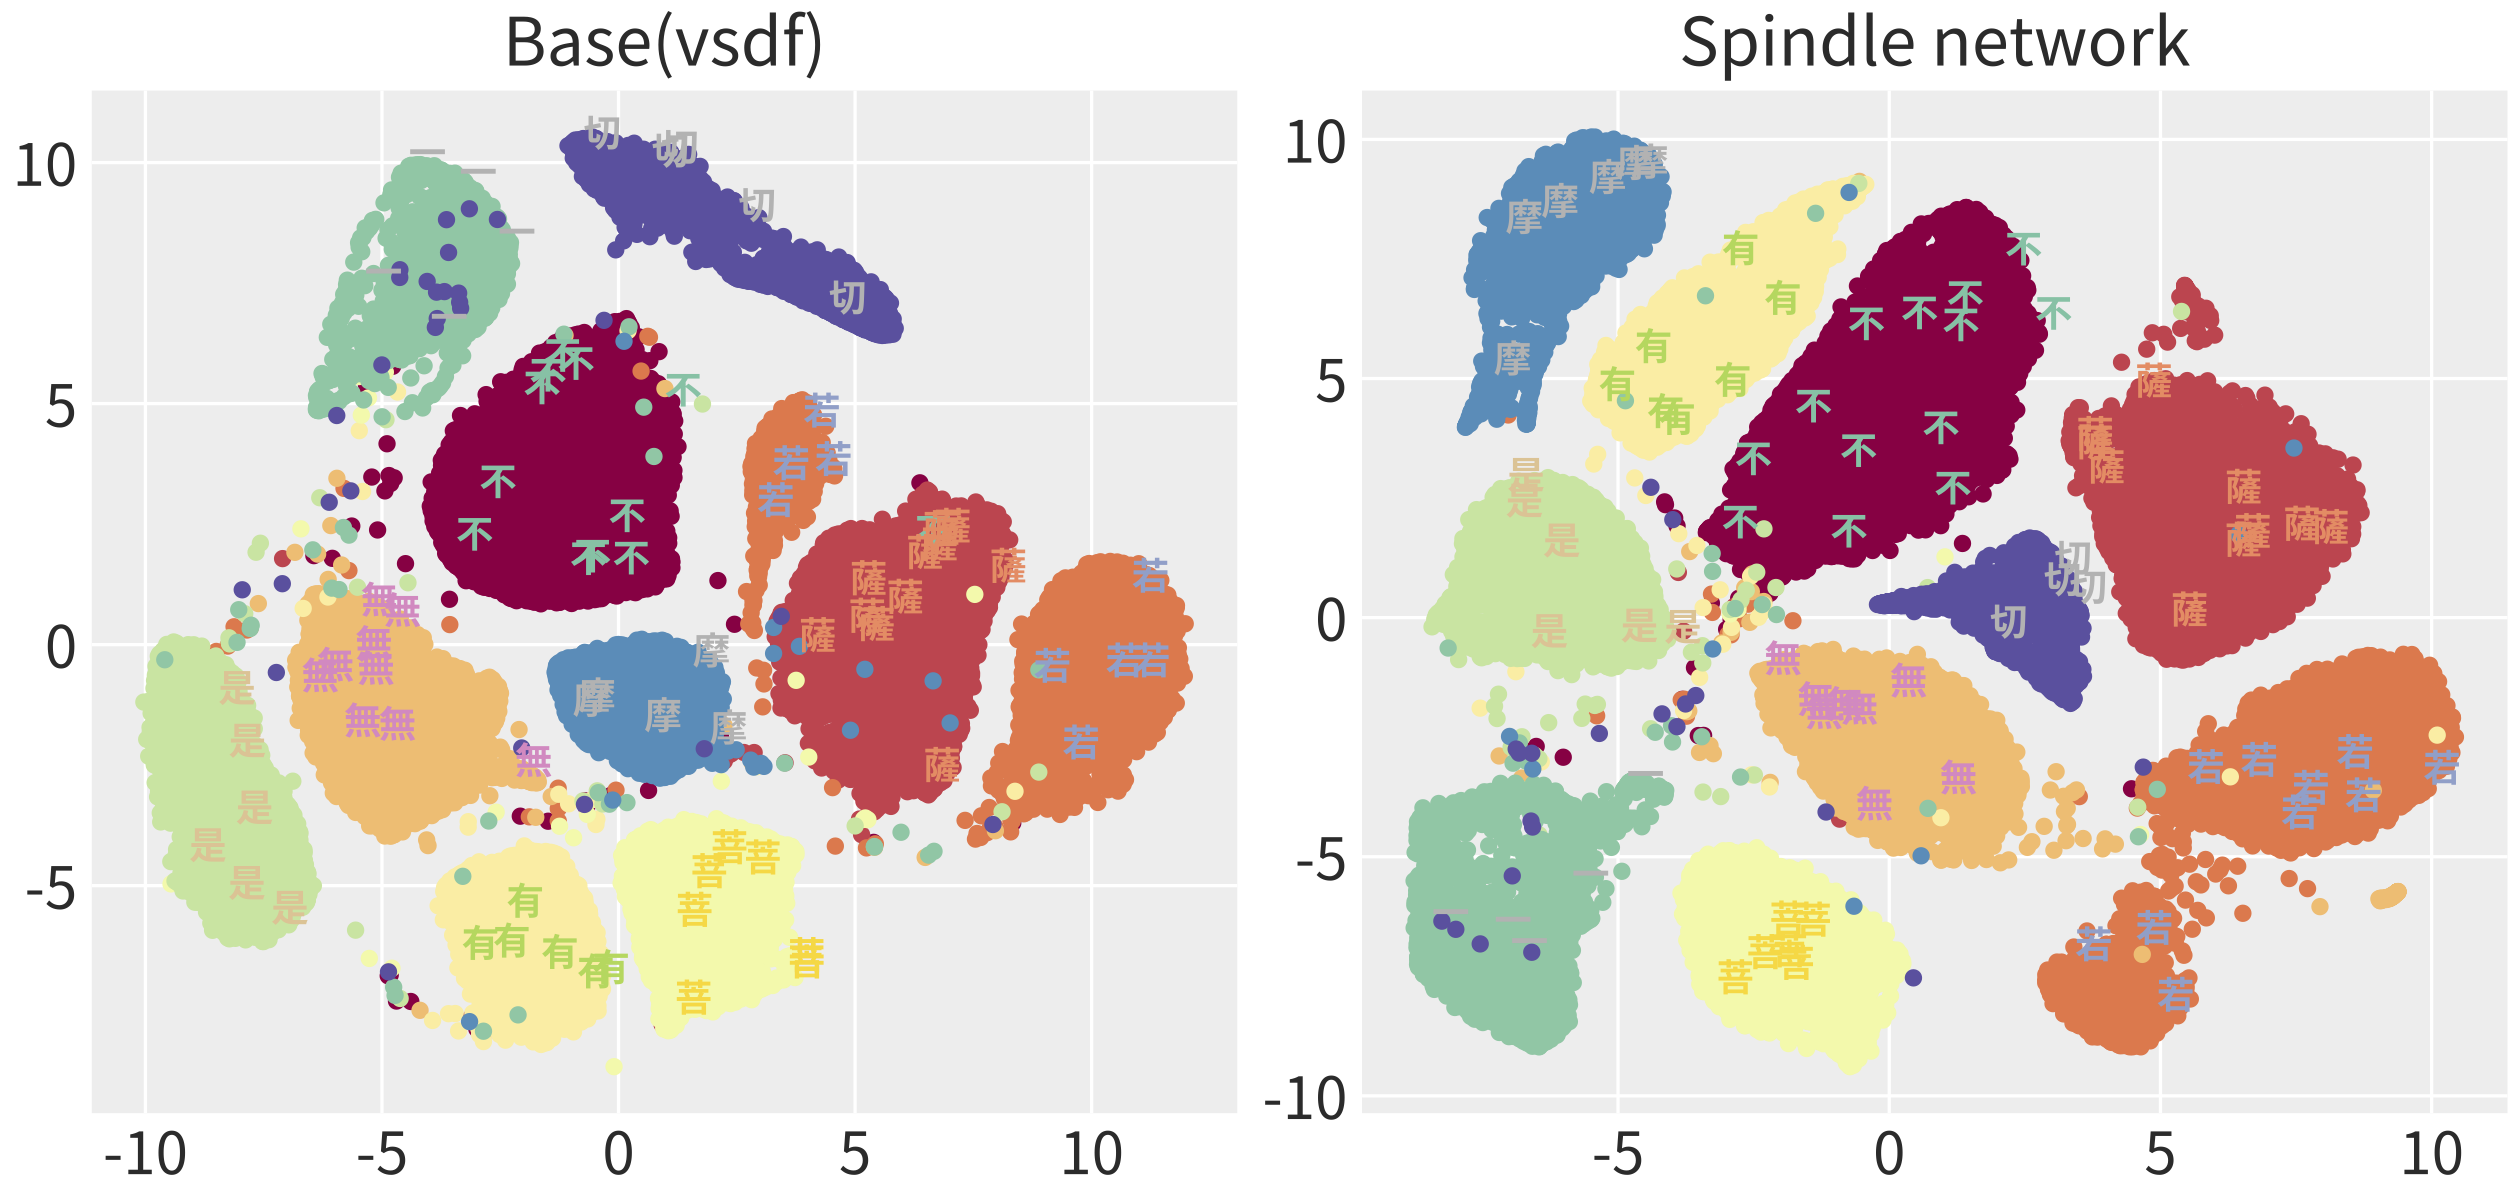
\includegraphics[width=1.0\linewidth]{figures/tsne.pdf}
    \end{center}
    \caption{Visualization of TSNE features from the top 10 character frequencies.}
    \label{fig:tsne}
\end{figure}

    
We further perform qualitative analysis to find out how the spindle net affects the character features, shown in Fig.\ref{fig:tsne}. In Fig.\ref{fig:tsne}, the tsne-cuda tool is used to visualize the last layer of features of the feature extractor. It can be seen that the features extracted by SpindleNet have clearer classification boundaries. For example, the orange character is divided into two  in base, while it is gathered together in SpindleNet. This shows that SpindleNet has better feature extraction capabilities.

\subsubsection{Architecture-level Ablative}
% In this section, we first demonstrate how the spindle-ness affects the performance. Then we discuss the structural sensitivity, i. e. which convolution layer deserves the most parameters. We first define the term ``spindle-ness'' by the largest channel number, % please change this one. and then perform quantitative analysis on the relation between the ``spindle-ness'' and the model performance.
% The results are shown in Fig.\ref{fig:spindleness}, ... % insert your analysis here.
\input{figures/archabl}
In this section, we discuss structural sensitivity, i.e.\ which convolutional layer deserves the most parameters. Fig.\ref{fig:archabl} shows the impact of structures on performance in two extreme cases, one is an equilateral triangle structure used in base, and the other is an inverted triangle structure. In the end, SpindleNet achieved the best results, which proves that appropriately increasing the number of channels or parameters in the head can improve model performance.

% We then analyze the structural sensitivity, i.e., which layer needs the most parameters. The results are shown in Fig.\ref{fig:archabl}. ... % insert your analysis here.
